\section{Experiments on a laboratory shaker - Test 2}
In the previous section, the first test on the shaker was presented. The test shown the capability of the framework to detect unknown harmonics. A second test was done to evaluate the capability to detect time domain variations and the effect of reducing the frequency resolution. The new configuration has been set to use only 4 frequency-domain features and the same 3 time-domain features of the previous test, for a total of 7 features. The signal used for training and testing are resumed in \autoref{tab:shaker_param_02}. It is the same signal at different amplitudes used for training and testing, plus another signal with different frequency content but the same amplitude as a training signal used for testing. 

The training has been carried out in the same way of the previous test, the training of the K-means model has been done with 4 clusters, and loaded on the microcontroller. The result of the novelty detection is shown in \autoref{fig:shaker_results02}. The forst 4 lines has been correctly identified as normal, as they was in fact a repetition of the training signals.
Then the purple and cyan line in the figure is the same signal, but 20 mV higher in amplitude \gls{wrt} the training signal. The novelty metric overshoots the threshold in 5 samples out of 20, so an increase of 2\% in amplitude generates the \gls{nd} event 25\% of the times. 

The brown, grey and green lines are the same signal, but with a bigger difference in amplitude \gls{wrt} the training signal. All the snapshots of theese signals correctly generated a novelty metric above the treshold. The blue line is the signal with a different frequency content, and it has been correctly identified as a novelty event, this is the confirmation that even with just 4 frequency bins, the wavelet decomposition is still generating features that are informative.

\todo % coommentare la linea azzurra


\begin{table}
    \centering
    \caption{Parameters of the second shaker test.}
    \label{tab:shaker_param_02}
    \begin{tabular}{cccccccc} 
    \toprule
    \multicolumn{5}{c}{\textbf{Harmonic frequency} {[}Hz]} & \multirow{2}{*}{\textbf{Amplitude }{[}mV$_{pp}$]} & \multicolumn{2}{c}{\textbf{ No. of snapshots}} \\
    10 & 30 & 60 & 70 & 100 &  & Train & Test \\ 
    \hline
    - & 0.1 & - & 1.0 & 1.0 & 580 & 100 & 10 \\
    - & 0.1 & - & 1.0 & 1.0 & 1000 & 100 & 10 \\
    - & 0.1 & - & 1.0 & 1.0 & 1980 & 100 & 10 \\
    - & 0.1 & - & 1.0 & 1.0 & 1540 & 100 & 10 \\
    - & 0.1 & - & 1.0 & 1.0 & 2000 & - & 20 \\
    - & 0.1 & - & 1.0 & 1.0 & 0 & - & 10 \\
    - & 0.1 & - & 1.0 & 1.0 & 800 & - & 10 \\
    - & 0.1 & - & 1.0 & 1.0 & 200 & - & 10 \\
    - & 0.1 & - & 1.0 & 1.0 & 1220 & - & 10 \\
    1.0 & 1.0 & 0.1 & - & - & 1540 & - & 10 \\
    \bottomrule
    \end{tabular}
    \end{table}

\begin{figure}
    \centering
    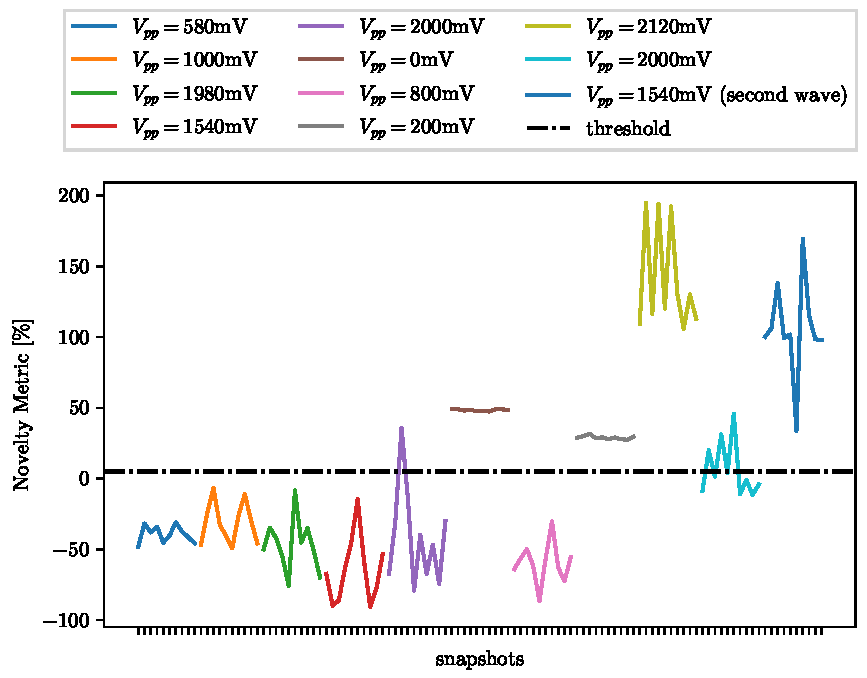
\includegraphics{Images/shaker/Test02.pdf}
    \caption{Novelty detection result}
    \label{fig:shaker_results02}
\end{figure}

\begin{figure}
    \centering
    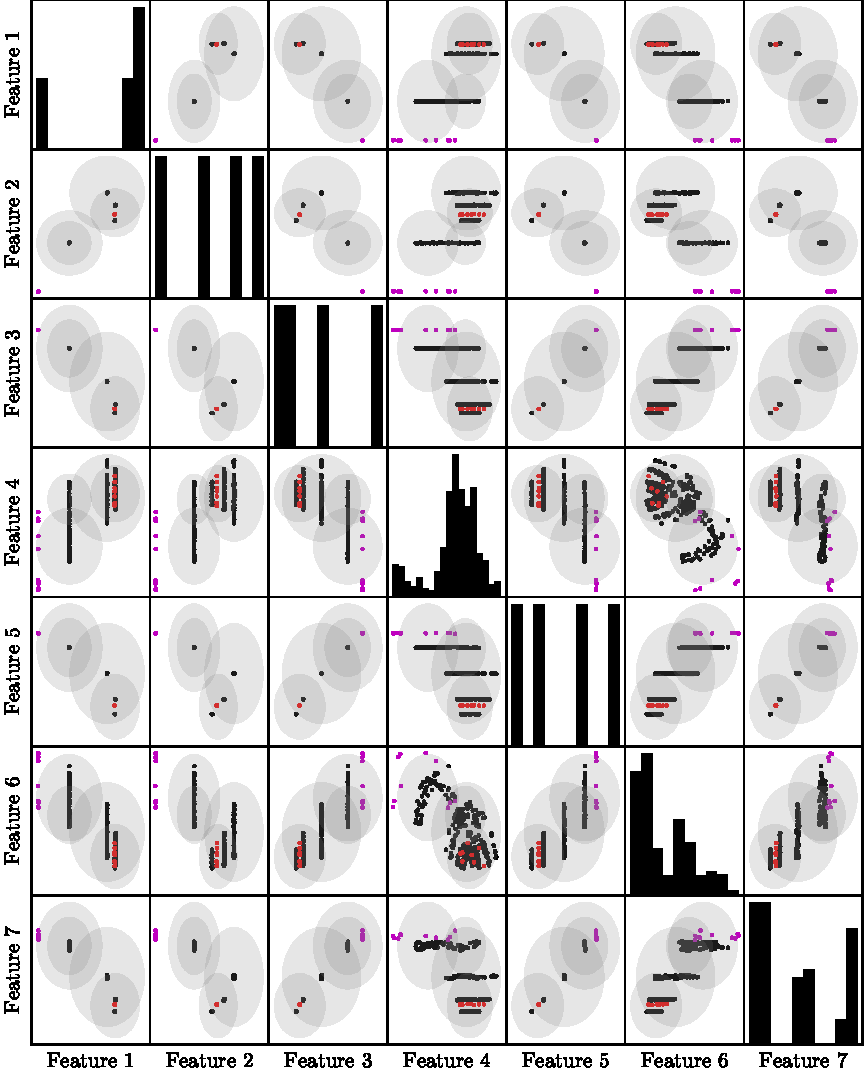
\includegraphics{Images/shaker/ConfusionMatrix.pdf}
    \caption{False Negative and True Positive results. On the diagonal, there is an histogram of the feature values. The off-diagonal plots are the scatter plots of the features. The shades are the projection of the clusters on the considered plane. (Red: False Negative, Magenta: True Positive, Black: training data)}
    \label{fig:shaker_conf_matrix}
    \end{figure}